\titre{11}
\theme{trigo}
\auteur{Nathan Scheinmann}
\niveau{1M}
\source{sesamath-1M-trigo}
\type{serie}
\piments{2}
\pts{}
\annee{2425}

\contenu{
\tcblower
\begin{minipage}[t]{0.5\textwidth}{
\vspace{0pt}
$SABCD$ est une pyramide régulière dont la base est le carré $ABCD$ de côté $230~\text{m}$ et de centre $I$. La hauteur $[SI]$ de la pyramide a pour longueur $\overline{SI}=147~\text{m}$. $M$ est le milieu de $[BC]$. 
}
\end{minipage}
\hfill
\begin{minipage}[t]{0.45\textwidth}{
\vspace{0pt}
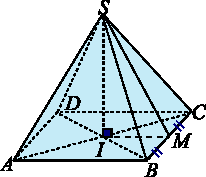
\includegraphics[scale=1.2]{../medias/1M/trigo/1M-exo-11}
}
\end{minipage}
\begin{tasks}
	\task Calculer le volume de la pyramide. 
	\task Calculer les mesures des angles $\widehat{IAS}$ et $\widehat{SMI}$ arrondies au degré près. 
\end{tasks}
}
\correction{

}

